\documentclass[12pt, a4paper, oneside]{ctexart}
\usepackage{amsmath, amsthm, amssymb, bm, graphicx, hyperref, mathrsfs}

\title{\textbf{Homework 4: Interpolation}}
\date{\today}
\linespread{1.5}
\begin{document}

\maketitle


\section{Step}
\begin{itemize}
    \item \textbf{代码编译:} 将代码编译成可执行文件,代码首先生成了一系列点的坐标,再使用三色样条插值法生成这些点之间的点,完成图像拟合。 
    \item \textbf{程序运行:} 运行可执行文件,生成一系列坐标点。
    \item \textbf{图形渲染:} 使用plotutils工具,根据生成的坐标点,渲染函数图像。
    
\end{itemize}
\section{Result}
    \begin{figure}[ht]
    \centering
    \includegraphics[width=0.5\textwidth]{./interp.eps}
    \caption{三色样条插值法拟合图像}
    \end{figure}
\end{document}